%-----------------------------------------------------------------------------
%
%               Template for sigplanconf LaTeX Class
%
% Name:         sigplanconf-template.tex
%
% Purpose:      A template for sigplanconf.cls, which is a LaTeX 2e class
%               file for SIGPLAN conference proceedings.
%
% Author:       Paul C. Anagnostopoulos
%               Windfall Software
%               978 371-2316
%               paul@windfall.com
%
% Created:      15 February 2005
%
%-----------------------------------------------------------------------------


\documentclass[preprint]{sigplanconf}

% The following \documentclass options may be useful:
%
% 10pt          To set in 10-point type instead of 9-point.
% 11pt          To set in 11-point type instead of 9-point.
% authoryear    To obtain author/year citation style instead of numeric.

\usepackage{ifthen}
\usepackage{fancyvrb}
\usepackage{color}
\usepackage{ulem}
\usepackage{xspace}
\usepackage{epsfig}
\usepackage{amssymb}
\usepackage{amsmath}
\usepackage{amsfonts}
\usepackage[utf8]{inputenc}
\usepackage{setspace}
\usepackage{relsize}

\usepackage{listings}

\usepackage[T1]{fontenc}
\usepackage{setspace}
\usepackage{listings}
\usepackage{beramono}

\definecolor{gray}{rgb}{0.3,0.3,0.3}

\lstset{
  basicstyle=\setstretch{1.05}\ttfamily\footnotesize,
  language=Python,
  keywordstyle=\bfseries,
  stringstyle=\color{blue},
  commentstyle=\color{gray}\textit,
  fancyvrb=true,
  showstringspaces=false,
  %keywords={def,while,if,elif,return,class,get,set,new,guard_class}
  numberstyle = \tiny,
  numbersep = -20pt,
}


\newboolean{showcomments}
\setboolean{showcomments}{true}
\ifthenelse{\boolean{showcomments}}
  {\newcommand{\nb}[2]{
    \fbox{\bfseries\sffamily\scriptsize#1}
    {\sf\small$\blacktriangleright$\textit{#2}$\blacktriangleleft$}
   }
   \newcommand{\version}{\emph{\scriptsize$-$Id: main.tex 19055 2008-06-05 11:20:31Z cfbolz $-$}}
  }
  {\newcommand{\nb}[2]{}
   \newcommand{\version}{}
  }

\newcommand\cfbolz[1]{\nb{CFB}{#1}}
\newcommand\arigo[1]{\nb{AR}{#1}}
\newcommand\fijal[1]{\nb{FIJAL}{#1}}
\newcommand\david[1]{\nb{DAVID}{#1}}
\newcommand\anto[1]{\nb{ANTO}{#1}}
\newcommand\reva[1]{\nb{Reviewer 1}{#1}}
\newcommand\revb[1]{\nb{Reviewer 2}{#1}}
\newcommand\revc[1]{\nb{Reviewer 3}{#1}}
\newcommand\revd[1]{\nb{Reviewer 4}{#1}}
\newcommand{\commentout}[1]{}
\newcommand{\ignore}[1]{} % {{\tt \small ignore(#1)}}

\newcommand\ie{i.e.,\xspace}
\newcommand\eg{e.g.,\xspace}
\newcommand{\etal}{\emph{et al.}\xspace}

\normalem

\let\oldcite=\cite

\renewcommand\cite[1]{\ifthenelse{\equal{#1}{XXX}}{[citation~needed]}{\oldcite{#1}}}


\begin{document}

\conferenceinfo{IWTC '11}{XXX} 
\copyrightyear{2011} 
\copyrightdata{[to be supplied]} 

\titlebanner{draft}        % These are ignored unless
%\preprintfooter{short description of paper}   % 'preprint' option specified.

\title{Loop-Aware Optimizations in PyPy's Tracing JIT}
%\subtitle{Subtitle Text, if any}

\authorinfo{H\aa kan Ardö}
           {Centre for Mathematical Sciences, Lund University}
           {hakan@debian.org}
\authorinfo{Carl Friedrich Bolz}
           {Heinrich-Heine-Universität Düsseldorf}
           {cfbolz@gmx.de}
\authorinfo{Maciej Fijałkowski}
           {}
           {fijall@gmail.com}

\maketitle

\begin{abstract}
One of the nice properties of a tracing JIT is that many of its optimization
are simple requiring one forward pass only. This is not true for loop-invariant code
motion which is a very important optimization for code with tight kernels.
In this paper we present a scheme for making simple optimizations loop-aware by
using a simple pre-processing step on the trace and not changing the
optimizations themselves. The scheme can give performance improvements of a
factor over two for PyPy's Python JIT executing simple numerical kernels
bringing the performance close to that of compiled C code.
\end{abstract}

\category{D.3.4}{Programming Languages}{Processors}[code generation,
incremental compilers, interpreters, run-time environments]

\terms
Languages, Performance, Experimentation

\keywords{Tracing JIT, Optimization, Loop-Invariant Code Motion}

\section{Introduction}

\reva{
You often use the word simple. While it might make sense to use it,
it exact meaning in that context remains unclear.
}

One of the advantages that tracing JIT compilers have above traditional
method-based
JITs is that their optimizers are much easier to write. Because a tracing JIT
produces only linear pieces of code without control flow joins, many
optimization passes on traces can have a very simple structure. They often
consist of one forward pass replacing operations by simpler ones or even
discarding them as they walk along it. This makes
optimization of traces very similar to symbolic execution. Also, many
difficult problems in traditional optimizers become tractable if the optimizer
does not need to deal with control flow merges.

One disadvantage of this simplicity is that such simple forward-passing
optimizers ignore the only bit of control flow they have available, which is
the fact that most traces actually represent loops. Making use of this
information is necessary to perform optimizations that take the whole loop into
account, such as loop-invariant code
motion or optimizations that improve across several iterations of the loop.
Having to deal with this property of traces complicates the optimization passes,
as a more global view of a trace needs to be considered when optimizing.

In this paper we want to address this problem by proposing a simple scheme that
makes it possible to turn optimizations using one forward pass into
optimizations that can do loop invariant code motion and similar loop-aware
improvements. Using this scheme one does not need to change the underlying
optimization much to get these advantages.

The resulting optimizations one gets using this scheme are in no way novel, most
of them are well-known loop optimizations. However, the way to implement them is
a lot simpler than directly implementing loop-aware optimizations.

% loop peeling does a lot more than loop-invariant code motion
% take this loop as an example:
% [i1, i2]
% i3 = i1 + 1
% i4 = i2 + 1
% escape(i4)
% jump(i2, i3)
% none of the operations is loop-invariant, but loop peeling will still remove the second addition

\section{Background: PyPy}
\label{sec:PyPy}

The work described in this paper was done in the context of the PyPy
project\footnote{\texttt{http://pypy.org}}. PyPy is a framework for implementing
dynamic languages efficiently \cite{armin_rigo_pypys_2006}. When implementing a
language with PyPy, one writes an interpreter for the language in RPython
\cite{davide_ancona_rpython:_2007}. RPython (``Restricted Python``) is a subset
of Python chosen in such a way that it can be efficiently translated to a
C-based VM by performing type inference.

Many low-level aspects of the final VM are not contained within the interpreter
implementation but are inserted during translation to C. Examples for this are a
garbage collector and also a tracing JIT compiler \cite{bolz_tracing_2009}.

PyPy's tracing JIT compiler traces on the level of RPython programs. Thus it
actually traces the execution of an interpreter written in RPython, not of the
program itself. This makes the details of the object model of the implemented
language transparent and optimizable by the tracing JIT. In the context of this
paper, this aspect of PyPy's tracing JIT can be ignored. Instead, it is
sufficient to view PyPy's tracing JIT as a JIT for RPython.


% section PyPy (end)

\section{Motivation}
\label{sec:Motivation}

\revc{
Don't break code listings across pages, as at the start of section 3.  It makes
them very hard to follow.
}

To motivate the approach we propose here, let's look at a trivial (unrealistic)
trace which corresponds to an infinite loop:

\begin{lstlisting}[mathescape,numbers = right,basicstyle=\setstretch{1.05}\ttfamily\scriptsize]
$L_0$($i_{0}$):
$i_1$ = $i_0$ + 1
print($i_1$)
jump($L_0$, $i_0$)
\end{lstlisting}

The first line is a label $L_0$ with argument $i_0$. Every label has a list of
arguments. The \lstinline{print} operation just prints its argument (it is not
an operation that PyPy's tracing JIT really supports, we just use it for this
example). The \lstinline{jump} operation jumps back to the beginning of the
trace, listing the new values of the arguments of the trace. In this case, the
new value of $i_0$ is $i_0$, making it a loop-invariant.

Because $i_0$ is loop-invariant, the addition could be moved out of the loop.
However, we want to get this effect using our existing optimization passes
without changing them too much. Simple optimizations with one forward pass
cannot directly get this effect: They just look at the trace without taking
into account that the trace executes many times in a row. Therefore to achieve
loop-invariant code motion, we peel one iteration off the loop before running
the optimizations. This peeling gives the following trace:

\begin{lstlisting}[mathescape,numbers = right,basicstyle=\setstretch{1.05}\ttfamily\scriptsize]
$L_0$($i_{0}$):
$i_1$ = $i_0$ + 1
print($i_1$)
jump($L_1$, $i_0$)

$L_1$($i_{0}$):
$i_2$ = $i_0$ + 1
print($i_2$)
jump($L_1$, $i_0$)
\end{lstlisting}

The iteration of the loop that was peeled off (lines 1-4) is called the
\emph{preamble}, the loop afterwards (lines 6-9) the \emph{peeled loop}.

Now the optimizer optimizes both of these two iterations of the loop together,
disregarding the \lstinline{jump} and the label in lines 4-6. Doing this, common
subexpression elimination will discover that the two additions are the same, and
replace $i_2$ with $i_1$. This leads to the following trace:

\begin{lstlisting}[mathescape,numbers = right,basicstyle=\setstretch{1.05}\ttfamily\scriptsize]
$L_0$($i_{0}$):
$i_1$ = $i_0$ + 1
print($i_1$)
jump($L_1$, $i_0$)

$L_1$($i_{0}$):
print($i_1$)
jump($L_1$, $i_0$)
\end{lstlisting}

This trace is malformed, because $i_1$ is used after the label $L_1$ without
being passed there, so we need to add $i_1$ as an argument to the label and pass
it along the \lstinline{jump}s:

\begin{lstlisting}[mathescape,numbers = right,basicstyle=\setstretch{1.05}\ttfamily\scriptsize]
$L_0$($i_{0}$):
$i_1$ = $i_0$ + 1
print($i_1$)
jump($L_1$, $i_0$, $i_1$)

$L_1$($i_{0}$, $i_1$):
print($i_1$)
jump($L_1$, $i_0$, $i_1$)
\end{lstlisting}

The final result is that the loop-invariant code was moved out of the loop into
the peeled-off iteration. Thus the addition is only executed in the first
iteration, while the result is reused in all further iterations.

This scheme is quite powerful and generalizes to other optimizations than just
common subexpression elimination. It allows simple linear optimization passes to
perform loop-aware optimizations, such as loop-invariant code motion without
changing them at all. All that is needed is to peel off one iteration, then
apply simple one-pass optimizations and make sure that the necessary extra
arguments are inserted into the label of the loop itself and the jumps
afterwards.

This is the key insight of the proposed implementation scheme: Giving an
optimization two iterations together at the same time gives the optimization
enough context to remove operations from the peeled loop, because it detects
that the operation was performed in the preamble already. Thus at runtime these
moved operations are only executed once when entering the loop and the results
are reused in further iterations.


% section Motivation (end)

\section{Running Example}
\label{sub:example}

\reva{
I think the motivation section is great, in particular for readers
who are less familiar with compiler/JIT optimizations. However,
section 4 starts with "yet another example" - at least this was my
impression when reading it. I understand the differences and
everything, but still, you might consider to improve the transition
between sections 3 and 4.
}

For the purpose of this paper, we are going to use a tiny interpreter for a dynamic language with
 a very simple object
model, that just supports an integer and a float type (this example has been taken from a previous paper \cite{bolz_allocation_2011}). The objects support only
one operation, \lstinline{add}, which adds two objects (promoting ints to floats in a
mixed addition). The implementation of \lstinline{add} uses classical Smalltalk-like
double-dispatching.
%These classes could be part of the implementation of a very
%simple interpreter written in RPython.
The classes can be seen in
Figure~\ref{fig:objmodel} (written in RPython).

\begin{figure}
\begin{lstlisting}[mathescape,basicstyle=\setstretch{1.05}\ttfamily\scriptsize]
class Base(object):
   pass

class BoxedInteger(Base):
   def __init__(self, intval):
      self.intval = intval

   def add(self, other):
      return other.add__int(self.intval)

   def add__int(self, intother):
      return BoxedInteger(intother + self.intval)

   def add__float(self, floatother):
      floatvalue = floatother + float(self.intval)
      return BoxedFloat(floatvalue)


class BoxedFloat(Base):
   def __init__(self, floatval):
      self.floatval = floatval

   def add(self, other):
      return other.add__float(self.floatval)

   def add__int(self, intother):
      floatvalue = float(intother) + self.floatval
      return BoxedFloat(floatvalue)

   def add__float(self, floatother):
      return BoxedFloat(floatother + self.floatval)


def f(y):
   step = BoxedInteger(-1)
   while True:
      y = y.add(step)
\end{lstlisting}
\caption{An ``Interpreter'' for a Tiny Dynamic Language Written in RPython}
\label{fig:objmodel}
\end{figure}

Using these classes to implement arithmetic shows the basic problem of many
dynamic language implementations. All the numbers are instances of either
\lstinline{BoxedInteger} or \lstinline{BoxedFloat}, therefore they consume space on the
heap. Performing many arithmetic operations produces lots of garbage quickly,
putting pressure on the garbage collector. Using double dispatching to
implement the numeric tower needs two method calls per arithmetic operation,
which is costly due to the method dispatch.

Let us now consider a simple ``interpreter'' function \lstinline{f} that uses the
object model (see the bottom of Figure~\ref{fig:objmodel}).
Simply running this function is slow, because there are lots of virtual method
calls inside the loop, two for each
call to \lstinline{add}. These method calls need to check the type of the involved
objects every iteration. In addition, a lot of objects are created
when executing that loop, many of these objects are short-lived.
The actual computation that is performed by \lstinline{f} is simply a sequence of
float or integer additions (note that \lstinline{f} does not actually terminate,
but it is still instructive to look at the produced traces).


\begin{figure}
\begin{lstlisting}[mathescape,numbers = right,basicstyle=\setstretch{1.05}\ttfamily\scriptsize]
$L_0$($p_{0}$, $p_{1}$):
# inside f: y = y.add(step)
guard_class($p_{1}$, BoxedInteger)
    # inside BoxedInteger.add
    $i_{2}$ = get($p_{1}$, intval)
    guard_class($p_{0}$, BoxedInteger)
        # inside BoxedInteger.add__int
        $i_{3}$ = get($p_{0}$, intval)
        $i_{4}$ = $i_{2} + i_{3}$
        $p_{5}$ = new(BoxedInteger)
            # inside BoxedInteger.__init__
            set($p_{5}$, intval, $i_{4}$)
jump($L_0$, $p_{0}$, $p_{5}$)
\end{lstlisting}
\caption{An Unoptimized Trace of the Example Interpreter}
\label{fig:unopt-trace}
\end{figure}

If the function is executed using the tracing JIT, with \lstinline{y} being a
\lstinline{BoxedInteger}, the produced trace looks like the one of
Figure~\ref{fig:unopt-trace} (lines starting with a hash ``\#'' are comments).
The trace corresponds to one iteration of the while-loop in \lstinline{f}.

The operations in the trace are indented
corresponding to the stack level of the function that contains the traced
operation. The trace is in single-assignment form, meaning that each variable is
assigned a value exactly once. The arguments $p_0$ and $p_1$ of the loop correspond
to the live variables \lstinline{y} and \lstinline{step} in the while-loop of
the original function.

The label of the loop is $L_0$ and is used by the jump instruction to
identify it's jump target.

The operations in the trace correspond to the operations in the RPython program
in Figure~\ref{fig:objmodel}:

\begin{itemize}
    \item \lstinline{new} creates a new object.
    \item \lstinline{get} reads an attribute of an object.
    \item \lstinline{set} writes to an attribute of an object.
    \item \lstinline{guard_class} is a precise type check. It typically precedes
    an (inlined) method call and is followed by the trace of the called method.
\end{itemize}

Method calls in the trace are preceded by a \lstinline{guard_class}
operation, to check that the class of the receiver is the same as the one that
was observed during tracing.\footnote{\lstinline{guard_class}
performs a precise
class check, not checking for subclasses.} These guards make the trace specific
to the situation where \lstinline{y} is really a \lstinline{BoxedInteger}. When
the trace is turned into machine code and afterwards executed with
\lstinline{BoxedFloat}, the
first \lstinline{guard_class} instruction will fail and execution will continue
using the interpreter.

\section{Making Trace Optimizations Loop Aware}

\revc{
In general, the paper is over-long on generalities and too short on details.
For example, the description of the basic technique at the beginning of section
5 is the third time the idea is explained at basically the same level of detail
(the others are in section 2 and section 4).  In contrast, the optimizations
applied rely on a simple type analysis, but this is only briefly alluded to.
}

Before a trace is passed to the backend compiling it into machine code
it is optimized to achieve better performance.
One goal of that is to move 
operations out of the loop making them executed only once
and not every iteration. This we propose to achieve by loop peeling. It
leaves the loop body intact, but prefixes it with one iteration of the
loop. This operation by itself will not achieve anything. But if it is
combined with other optimizations it can increase the effectiveness of
those optimizations. For many optimization of interest only a few
additional details has to be considered when they are combined with loop peeling. These are
described below by explaining the loop peeling optimization
followed by a set of other optimizations and how they interact with
loop peeling.

\subsection{Loop Peeling}

\begin{figure}
\begin{center}
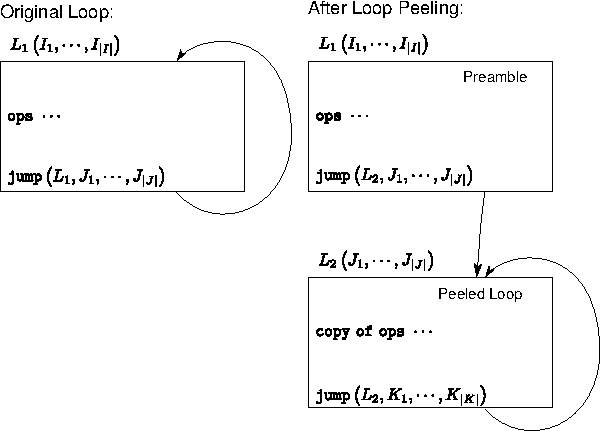
\includegraphics[width=\columnwidth]{figures/overview}
\end{center}
\caption{Overview of Loop Peeling}
\label{fig:overview}
\end{figure}

Loop peeling is achieved by appending an copy of the traced iteration at
the end of itself. See Figure~\ref{fig:overview} for an illustration.
The first part (called \emph{preamble}) finishes with a jump the the second part
(called the \emph{peeled loop}). The second part finishes with a jump to itself. This way
the preamble will be executed only once while the peeled loop will
be used for every further iteration. New variable names have to be
introduced in the entire copied trace in order to maintian the SSA-property.
Note that the peeled loop is not necessary the \emph{first} iteration of the
loop execution, it is general enough to correspond to any iteration of the loop.
However, the peeled loop can then be optimized using the assumption that a
previous iteration has happened.

%XXX (samuele): the point about the first iteration is hard to understand

When applying optimizations to this two-iteration trace
some care has to taken as to how the arguments of the two
\lstinline{jump} operations and the input arguments of the peeled loop are
treated. It has to be ensured that the peeled loop stays a proper
trace in the sense that the operations within it only operates on
variables that are either among its input arguments 
or produced within the peeled loop. To ensure this we need
to introduce a bit of formalism.

The original trace (prior to peeling) consists of three parts.
A vector of input
variables, $I=\left(I_1, I_2, \cdots, I_{|I|}\right)$, a list of non-
jump operations and a single
jump operation. The jump operation contains a vector of jump variables,
$J=\left(J_1, J_2, \cdots, J_{|J|}\right)$, that are passed as the input variables of the target loop. After
loop peeling there will be a second copy of this trace with input
variables equal to the jump arguments of the preamble, $J$, and jump
arguments $K$. 
Figure~\ref{fig:overview} illustrates the general case. The running
example in Figure~\ref{fig:unopt-trace} has  $I = \left( p_0, p_1
\right)$ and $J = \left( p_0, p_5 \right)$. The result of applying
loop peeling to it is shown in Figure~\ref{fig:peeled-trace} with 
$K = \left( p_0, p_9 \right)$. 

To construct the second copy of the trace (the peeled loop) from the
first (the preeamble) we need a
function $m$, mapping the variables of the preamble onto the
variables of the peeled loop. This function is constructed during the
copying. It is initialized by mapping the input arguments, $I$, to
the jump arguments $J$,
\begin{equation}
  m\left(I_i\right) = J_i \ \text{for}\ i = 1, 2, \cdots |I| .
\end{equation}
In the example that means:

\begin{equation}
  %\left\{
    \begin{array}{lcl}
      m\left(p_0\right) &=& p_0 \\
      m\left(p_1\right) &=& p_5
    \end{array}
  %\right.
  .
\end{equation}



Each operation in the trace is copied in order.
To copy an operation $v=\text{op}\left(A_1, A_2, \cdots, A_{|A|}\right)$
a new variable, $\hat v$ is introduced. The copied operation will
return $\hat v$ using
\begin{equation}
  \hat v = \text{op}\left(m\left(A_1\right), m\left(A_2\right), 
    \cdots, m\left(A_{|A|}\right)\right) . 
\end{equation}
Before the
next operation is copied, $m$ is extend by assigning $m\left(v\right) = \hat
v$. For the example above, that will extend $m$ with
\begin{equation}
  %\left\{
    \begin{array}{lcl}
      m\left(i_2\right) &=& i_6 \\
      m\left(i_3\right) &=& i_7 \\
      m\left(i_4\right) &=& i_8 \\
      m\left(p_5\right) &=& p_9 \\
    \end{array}
  %\right.
  .
\end{equation}

\begin{figure}
\begin{lstlisting}[mathescape,numbers = right,basicstyle=\setstretch{1.05}\ttfamily\scriptsize]
$L_0$($p_{0}$, $p_{1}$):
# inside f: y = y.add(step)
guard_class($p_{1}$, BoxedInteger)
    # inside BoxedInteger.add
    $i_{2}$ = get($p_{1}$, intval)
    guard_class($p_{0}$, BoxedInteger)
        # inside BoxedInteger.add__int
        $i_{3}$ = get($p_{0}$, intval)
        $i_{4}$ = $i_{2}+i_{3}$
        $p_{5}$ = new(BoxedInteger)
            # inside BoxedInteger.__init__
            set($p_{5}$, intval, $i_{4}$)
jump($L_1$, $p_{0}$, $p_{5}$)

$L_1$($p_{0}$, $p_{5}$):
# inside f: y = y.add(step)
guard_class($p_{5}$, BoxedInteger)
    # inside BoxedInteger.add
    $i_{6}$ = get($p_{5}$, intval)
    guard_class($p_{0}$, BoxedInteger)
        # inside BoxedInteger.add__int
        $i_{7}$ = get($p_{0}$, intval)
        $i_{8}$ = $i_{6}+i_{7}$
        $p_{9}$ = new(BoxedInteger)
            # inside BoxedInteger.__init__
            set($p_{9}$, intval, $i_{8}$)
jump($L_1$, $p_{0}$, $p_{9}$)
\end{lstlisting}
\caption{A peeled trace of the Example Interpreter}
\label{fig:peeled-trace}
\end{figure}

\section{Interaction of Optimizations with Loop Peeling}

\subsection{Redundant Guard Removal}

No special concerns needs to be taken when implementing redundant
guard removal together with loop peeling. The guards from
the preamble might make the guards of the peeled loop
redundant and thus removed. Therefore one effect of combining redundant
guard removal with loop peeling is that loop-invariant guards are moved out of the
loop. The peeled loop of the example reduces to

\begin{lstlisting}[mathescape,numbers = right,basicstyle=\setstretch{1.05}\ttfamily\scriptsize]
$L_1$($p_{0}$, $p_{5}$):
# inside f: y = y.add(step)
    # inside BoxedInteger.add
    $i_{6}$ = get($p_{5}$, intval)
        # inside BoxedInteger.add__int
        $i_{7}$ = get($p_{0}$, intval)
        $i_{8}$ = $i_{6}+i_{7}$
        $p_{9}$ = new(BoxedInteger)
            # inside BoxedInteger.__init__
            set($p_{9}$, intval, $i_{8}$)
jump($L_1$, $p_{0}$, $p_{9}$)
\end{lstlisting}

The guard on $p_5$ on line 17 of Figure~\ref{fig:peeled-trace} can be
removed since $p_5$ is allocated on line 10 with a known class. The
guard on $p_0$ on line 20 can be removed since it is identical to the
guard on line 6.

Note that the guard on $p_5$ is removed even though $p_5$ is not loop
invariant, which shows that loop invariant code motion is not the only
effect of loop peeling. Loop peeling can also remove guards that are implied by
the guards of the previous iteration.



\subsection{Common Subexpression Elimination and Heap Optimizations}

If a pure operation appears more than once in the trace with the same input
arguments, it only needs be executed the first time and then the result
can be reused for all other appearances. PyPy's optimizers can also remove
repeated heap reads if the intermediate operations cannot have changed their
value\footnote{We perform a simple type-based alias analysis to know which
writes can affect which reads. In addition writes on newly allocated objects
can never change the value of old existing ones.}.

When that is combined with loop peeling, the single execution of the operation
is placed in the preamble. That is, loop invariant pure operations and heap
reads are moved out of the loop. 

Consider the \lstinline{get} operation on line 22 of
Figure~\ref{fig:peeled-trace}. The result of this operation can be
deduced to be $i_3$ from the \lstinline{get} operation on line
8. The optimization will thus remove line 22 from the trace and
replace $i_7$ with $i_3$. Afterwards the trace is no longer in the correct
form, because the argument $i_3$ is not passed along the loop arguments. It
thus needs to be added there.

The trace from Figure~\ref{fig:peeled-trace} will therefore be optimized to:

\begin{lstlisting}[mathescape,numbers = right,basicstyle=\setstretch{1.05}\ttfamily\scriptsize]
$L_0$($p_{0}$, $p_{1}$):
# inside f: y = y.add(step)
guard_class($p_{1}$, BoxedInteger)
    # inside BoxedInteger.add
    $i_{2}$ = get($p_{1}$, intval)
    guard_class($p_{0}$, BoxedInteger)
        # inside BoxedInteger.add__int
        $i_{3}$ = get($p_{0}$, intval)
        $i_{4}$ = $i_{2}+i_{3}$
        $p_{5}$ = new(BoxedInteger)
            # inside BoxedInteger.__init__
            set($p_{5}$, intval, $i_{4}$)
jump($L_1$, $p_{0}$, $p_{5}$, $i_3$)

$L_1$($p_{0}$, $p_{5}$, $i_3$):
# inside f: y = y.add(step)
guard_class($p_{5}$, BoxedInteger)
    # inside BoxedInteger.add
    $i_{6}$ = get($p_{5}$, intval)
    guard_class($p_{0}$, BoxedInteger)
        # inside BoxedInteger.add__int
        $i_{8}$ = $i_{4}+i_{3}$
        $p_{9}$ = new(BoxedInteger)
            # inside BoxedInteger.__init__
            set($p_{9}$, intval, $i_{8}$)
jump($L_1$, $p_{0}$, $p_{9}$, $i_3$)
\end{lstlisting}

After loop peeling and redundant operation removal the peeled loop
will typically no longer be in SSA form but operate on variables that are the result
of operations in the preamble. The solution is to extend the input
arguments, $J$, with those variables. This will also extend the
jump arguments of the preamble, which is also $J$. 
Implicitly that also extends the jump arguments of the peeled loop, $K$,
since they are the image of $J$ under $m$. For the example $I$ has to
be replaced by $\hat I$ which is formed by appending $i_3$ to $I$.
At the same time $K$ has to be replaced by
$\hat K$ which is formed by appending $m\left(i_3\right)=i_7$ to $K$.
The variable $i_7$ will then be replaced by $i_3$ by the heap caching
optimization as it has removed the variable $i_7$.

In general what is needed is to keep track of
which variables from the preamble are reused in the peeled loop.
By constructing a vector, $H$,  of such variables, the input and jump
arguments can be updated using
\begin{equation}
  \hat J = \left(J_1, J_2, \cdots, J_{|J|}, H_1, H_2, \cdots, H_{|H}\right)
  \label{eq:heap-inputargs}
\end{equation}
and
\begin{equation}
  \hat K = \left(K_1, K_2, \cdots, K_{|J|}, m(H_1), m(H_2), \cdots, m(H_{|H})\right)
  .
  \label{eq:heap-jumpargs}
\end{equation}
In the optimized trace $I$ is replaced by $\hat I$ and $K$ by $\hat
K$.

\subsection{Allocation Removals}
\label{sub:allocation}

PyPy's allocation removal optimization \cite{bolz_allocation_2011} makes it
possible to identify objects that are allocated within the loop but never
escape it. That is, no outside
object ever gets a reference to them. This
is performed by processing the operations in order and
optimistically removing every \lstinline{new} operation. Later on if
it is discovered that a reference to the object escapes the loop, the
\lstinline{new} operation is inserted at this point. All operations
(\lstinline{get}, \lstinline{set} and \lstinline{guard}) on the removed objects
are also removed and the optimizer needs to keep track of the value of all used
attributes of the object.

Consider again the original unoptimized trace of
Figure~\ref{fig:peeled-trace}. Line 10 contains the first
allocation. It is removed and $p_5$ is marked as allocation-removed. This means
that it refers to an object that has not yet been
(and might never be) allocated. Line 12 sets the \lstinline{intval}
attribute of $p_5$. This operation is also removed and the optimizer
registers that the attribute \lstinline{intval} of $p_5$ is $i_4$.

When the optimizer reaches line 13 it needs to construct the
arguments of the \lstinline{jump} operation, which contains the
reference to the allocation-removed object in $p_5$. This can be achieved by
exploding $p_5$ into the attributes of the allocation-removed object.
In this case there is only one such attribute and its value is
$i_4$, which means that $p_5$ is replaced with $i_4$ in the jump
arguments. 

In the general case, each allocation-removed object in the jump arguments is exploded into a
vector of variables containing the values of all registered
attributes\footnote{This is sometimes called \emph{scalar replacement}.}.
If some of the attributes are themselves references to
allocation-removed objects they are recursively exploded
to make the vector contain only concrete variables. Some care has
to be taken to always place the attributes in the same order when
performing this explosion. Notation becomes somewhat simpler if also every
concrete variable of the jump arguments is exploded into a vector containing
itself. For
every variable, $J_k$, of the original jump arguments, $J$, let
\begin{equation}
  \tilde J^{\left(k\right)} = \left\{
      \begin{array}{ll}
        \left(J_k\right)  & \text{if $J_k$ is concrete} \\
        H^{\left(k\right)} & \text{if $J_k$ is allocation-removed}
      \end{array}
  \right.
  ,
\end{equation}
where $H^{\left(k\right)}$ is a vector containing all concrete
attributes of $J_k$. The arguments of the optimized \lstinline{jump}
operation are constructed as the concatenation all the $\tilde J^{\left(k\right)}$ vectors,
\begin{equation}
  \hat J = \left( 
    \begin{array}{cccc}
      \tilde J^{\left(1\right)} & \tilde J^{\left(2\right)} & \cdots &
      \tilde J^{\left(|J|\right)} \\
    \end{array}
  \right)      
  .
\end{equation}
The arguments of the \lstinline{jump} operation of the peeled loop,
$K$, is constructed by inlining $\hat J$,
\begin{equation}
  \hat K = \left(m\left(\hat J_1\right), m\left(\hat J_1\right), 
                 \cdots, m\left(\hat J_{|\hat J|}\right)\right)
  .
\end{equation}
In the optimized trace $I$ is replaced by $\hat I$ and $K$ by $\hat
K$. The trace from Figure~\ref{fig:unopt-trace} will be optimized into

\begin{lstlisting}[mathescape,numbers = right,basicstyle=\setstretch{1.05}\ttfamily\scriptsize]
$L_0$($p_{0}$, $p_{1}$):
# inside f: y = y.add(step)
guard_class($p_{1}$, BoxedInteger)
    # inside BoxedInteger.add
    $i_{2}$ = get($p_{1}$, intval)
    guard_class($p_{0}$, BoxedInteger)
        # inside BoxedInteger.add__int
        $i_{3}$ = get($p_{0}$, intval)
        $i_{4}$ = $i_{2}+i_{3}$
            # inside BoxedInteger.__init__
jump($L_1$, $p_{0}$, $i_{4}$)

$L_1$($p_{0}$, $i_{4}$):
# inside f: y = y.add(step)
    # inside BoxedInteger.add
    guard_class($p_{0}$, BoxedInteger)
        # inside BoxedInteger.add__int
        $i_{7}$ = get($p_{0}$, intval)
        $i_{8}$ = $i_{4}+i_{7}$
            # inside BoxedInteger.__init__
jump($L_1$, $p_{0}$, $i_8$)
\end{lstlisting}

If all the optimizations presented above are applied, the resulting
optimized peeled loop will consist of a single integer addition
only. That is it will become type-specialized to the types of the
variables \lstinline{step} and \lstinline{y}, and the overhead of
using boxed values is removed.

\revc{
This paper presents an elegant, if simple, technique, and demonstrates that
it's effective in small cases.  The worked example is particularly helpful, and
would be better if it were worked more thoroughly.  Some of the omitted steps
are not entirely obvious, and the paper would be improved by making the
clearer.  In particular, the final program presented on the bottom of page 5,
first column, still has memory access, boxing, and type checks, which the paper
then claims can be removed.  There's enough space to show this.
}

\section{Benchmarks}


\revb{
A nit: Section 7 says that loop peeling never makes runtime
performance worse, but generating more code can potentially slow
performance. I assume that non-numeric benchmarks show no slowdown in
practice, and that might be worth noting.
}

\revb{
Section 7 also mentions performance improvements for a Prolog
interpreter. Consider adding a brief explanation of the benefit, since
that example stands out as a non-numeric (I assume) performance
improvement.
}

\revc{
Providing source code for the benchmarks measured are needed for others to
reproduce and build on your results.  I believe this should be the minimum
standard for publishing measurements such as these.
}

\revc{
I would have liked to have benchmark results for some larger applications.
When is this optimization effective on a large scale, if ever?
}

\revd{
It isn't clear from the paper, but a reader might conclude that the bulk of the
time savings are from removing boxing/unboxing operations.
}

\revd{
The benchmark results appear quite impressive -- especially the comparison with
GCC -- but without additional information, I have no idea what is being
compared.  Are these results from the same sizes of integers and/or floating
point results?
}

\revd{
This paper is relatively short, and could be significantly improved with a
couple of pages of additional information about the details of the benchmarks
-- both on the Python and on the C side.
}

The loop peeling optimization was implemented in the PyPy
framework in about 450 lines of RPython code. That means that the JIT-compilers generated for all
interpreters implemented within PyPy now can take advantage of
it. Benchmarks have been executed for a few different interpreters and
we see improvements in several cases. The ideal loop for this optimization
is short and contains numerical calculations with no failing guards and no
external calls. Larger loops involving many operations on complex objects
typically benefit less from it. Loop peeling never makes runtime performance worse, in
the worst case the peeled loop is exactly the same as the preamble. Therefore we
chose to present benchmarks of small numeric kernels where loop peeling can show
its use.

\begin{figure}
\begin{center}
{\smaller
\begin{tabular}{|l|r|r|r|r|r|r|}
\hline
 & CPython & Psyco & PyPy  & PyPy & GCC \\
 &         &       & no LP &      & -O3 \\
\hline
conv3(1e5) & 77.89 & 9.52 & 1.77  & 0.68 &  0.59 \\
\hline
conv3(1e6) & 77.15 & 9.58 & 1.69  & 0.77 &  0.74 \\
\hline
conv3x3(1000) & 233.54 & 125.40 & 0.57 & 0.27 & 0.25 \\
\hline
conv3x3(3) & 234.45 & 126.28 & 0.60 & 0.31 & 0.28 \\
\hline
conv5(1e5) & 122.54 & 16.67 & 1.86  & 1.05 &  0.65\\
\hline
conv5(1e6) & 125.77 & 16.80 & 1.92 & 1.09 &  0.80 \\
\hline
dilate3x3(1000) & 232.51 & 125.85 & 3.89 & 3.69 & 0.25 \\
\hline
sobel(1000) & 181.49 & 95.05 & 0.71 & 0.42 & 0.20 \\
\hline
sqrt(Fix16) & 744.35 & 421.65 & 3.93  & 2.14  & 0.96 \\
\hline
sqrt(float) & 24.21 & 5.52 & 1.36 & 1.00 & 0.98\\
\hline
sqrt(int) & 20.84 & 1.78 & 2.26 & 1.82  & 0.80 \\
\hline
\hline
Variations & - & - & $\pm 0.03$ & $\pm 0.01$ & $\pm 0.01$ \\
\hline
\end{tabular}
}
\end{center}
\label{fig:benchmarks}
\caption{Benchmark Results in Seconds. Arrays of length $10^5$ and
  $10^6$ and matrixes of size $1000\times 1000$ and $1000000 \times
  3$ are used. The one used in each benchmark is indicated in
  the leftmost column. For the matrixes, only the number of rows are
  specified.} 
\end{figure}

\subsection{Python}
The Python interpreter of the PyPy framework is a complete Python
version 2.7 compatible interpreter. A set of numerical
calculations were implemented in both Python and in C and their
runtimes are compared in Figure~\ref{fig:benchmarks}. The benchmarks are
\begin{itemize}
\item {\bf sqrt}: approximates the square root of $y$ as $x_\infty$
  with $x_0=y/2$ and $x_k = \left( x_{k-1} + y/x_{k-1} \right) /
  2$. There are three different versions of this benchmark where $x_k$
  is represented with different type of objects: int's, float's and
  Fix16's. The latter, Fix16, is a custom class that implements
  fixpoint arithmetic with 16 bits precision. In Python there is only
  a single implementation of the benchmark that gets specialized
  depending on the class of it's input argument, $y$, while in C,
  there are three different implementations.
\item {\bf conv3}: one-dimensional convolution with fixed kernel-size $3$.
\item {\bf conv5}: one-dimensional convolution with fixed kernel-size $5$.
\item {\bf conv3x3}: two-dimensional convolution with kernel of fixed
  size $3 \times 3$ using a custom class to represent two-dimensional
  arrays.
\item {\bf dilate3x3}: two-dimensional dilation with kernel of fixed
  size $3 \times 3$. This is similar to convolution but instead of
  summing over the elements, the maximum is taken. That places a
  external call to a max function within the loop that prevents some
  of the optimizations.
\item {\bf sobel}: a low-level video processing algorithm used to
  locate edges in an image. It calculates the gradient magnitude
  using sobel derivatives. 
\end{itemize}

The sobel and conv3x3 benchmarks are implemented
on top of a custom two-dimensional array class.
It is
a simple straight forward implementation providing 2 dimensionall
indexing with out of bounds checks. For the C implementations it is
implemented as a C++ class. The other benchmarks are implemented in
plain C. 

Benchmarks were run on Intel i7 M620 @2.67GHz with 4M cache and 8G of RAM
using Ubuntu Linux 11.4 in 32bit mode.
The machine was otherwise unoccupied. We use the following software
for benchmarks:

\begin{itemize}
\item PyPy 1.5
\item CPython 2.7.2
\item Psyco 1.6 with CPython 2.6.6
\item GCC 4.4.5 shipped with Ubuntu 11.4
\end{itemize}

We run GCC both with -O2 optimization and -O3 -march=native, disabling the
automatic loop vectorization. In all cases, SSE2 instructions were used for
floating point operations, except Psyco which uses x87 FPU instructions.
We also run PyPy with loop peeling optimization and without (but otherwise
identical).

For PyPy 10 iterations were run, prefaced with 3 iterations for warming up.
Due to benchmarks taking large amounts of time on CPython, only one run
was performed, prefaced with one warmup run for Psyco.
For GCC 5 iterations
were run. In all cases, the standard deviation is very low, making benchmarks
very well reproducible.

We can observe that PyPy (even without loop peeling) is orders of magnitude
faster than either CPython or Psyco. This is due to the JIT compilation
advantages and optimizations we discussed in previous work
\cite{bolz_allocation_2011, bolz_runtime_2011}. The geometric mean of the
speedup of loop peeling is 70\%, which makes benchmark times
comparable with native-compiled C code. We attribute the performance gap to C code to
the relative immaturity of PyPy's JIT assembler backend as well as missing
optimizations, like instruction scheduling.

Other interesting interpreters that are helped greatly by this
optimization are for
example our Prolog interpreter written in RPython, as well as numerical
kernel used for array manipulation. The exact extent is out of scope for
this paper.

\section{Related Work}
\label{sec:related}

\reva{
First sentence of the related work section is kind of
unfortunate. It is unclear what the reference at the end of the
sentence is good for. To support the meaning of the entire sentence?
Or is it just a reference to the standard loop invariant code motion
techniques? The contribution of your paper seems much smaller than
in the former case compared to the latter one. While I have not
checked the content of the book, I believe the latter is the correct
interpretation. You should remove this opportunity for
misinterpretation.}

The effect of combining a one pass optimization with loop peeling gives
completely standard loop invariant code motion optimizations
\cite{muchnick_advanced_1997}. We do not claim any novelty in the effect, but
think that our implementation scheme is a very simple one.

\revc{
The discussion of LuaJIT is unsatisfying.  It's not clear to me from that one
quote that Mike is doing the same thing.  It might be worth including LuaJIT in
the benchmarks, and/or examining the actual implementation of LuaJIT.
}

Mike Pall, the author of LuaJIT\footnote{\texttt{http://luajit.org/}} seems to
have developped the described technique independently. There are no papers about
LuaJIT but the author of it writes on a mailing list: ``The LOOP pass does
synthetic unrolling of the recorded IR, combining copy-substitution with
redundancy elimination to achieve code hoisting. The unrolled and
copy-substituted instructions are simply fed back into the compiler pipeline,
which allows reuse of all optimizations for redundancy elimination. Loop
recurrences are detected on-the-fly and a minimized set of PHIs is generated.''
\cite{pall_luajit_2009}

Both the Hotpath VM \cite{gal_hotpathvm:_2006} and SPUR
\cite{bebenita_spur:_2010} implements loop-invariant code motion
directly, by explicitly marking as loop-invariant all variables that stay the
same along all looping paths and then moving all pure computation that depends
only on these variables out of the loop. SPUR can also hoist loads out of the
loop if nothing in the loop can ever write to the memory location. It can also
move allocations out of the loop, but does not replace the object by its attributes.
This saves only the allocation, not the access to the object attributes.

The type specialization described by Gal \etal \cite{gal_trace-based_2009} can
be seen as doing a similar optimization (again by manually implementing it)
than the one described in Section~\ref{sub:allocation}: The effect of both is
that type checks are fully done before a loop is even entered.


% section Related Work (end)

\section{Conclusions}

In this paper we have studied loop invariant code motion during trace
compilation. We claim that loop peeling is a very convenient solution
here since it fits well with other trace optimizations and does not require
large changes to them. This approach improves the effect of standard
optimizations such as redundant guard removal, common subexpression elimination
and allocation removal. The most prominent effect is that they all become loop
invariant code motion optimizations.

By using several benchmarks we show that the proposed algorithm can
significantly improve the run time of small loops containing numerical
calculations. 

The current approach still has some limitations which we plan to address in the
future. In particular loop peeling works poorly in combination with trace
trees or trace stitching. The side exits attached guards that fail often
currently have to jump to the preamble which makes loops with several equally
common paths less efficient than they could be.

%\appendix
%\section{Appendix Title}

%This is the text of the appendix, if you need one.

%\acks
%Acknowledgments, if needed.

% We recommend abbrvnat bibliography style.

\bibliographystyle{abbrv}
\bibliography{paper}

\end{document}
